\subsection{Chemotherapeutic drugs}
\subsubsection{Ibrutinib (Ibr)}
Ibrutinib (Ibr) is a chemotherapic drug (Fig. \ref{fig:Ibr}) used as a deactivator of Bruton tyrosine kinase (BTK), that acts as molecular mediator of pathogenesis and is essential for B cell receptor signaling\cite{ibr-1}.  
Whenever B cells receptor signaling has an aberrhant behaviour alongside antigen-dependent activation, is involved in the pathogenesis of many lymphocytes-related malignancies.\\
Ibr blocks B cell antigen receptor signalling through an irreversible covalent bond with Cys-481 of BTK, hence reducing malignant B cell proliferation and inducing cell death.\\
The drug reaches its maximum concentration in plasma ($953\,\text{ng}\cdot\text{h}/\text{mL}$ at dosage of $560\,\text{mg}/\text{day}$) in 1-2 h and is widely distributed in the body. The major route of elimination is metabolism. It is metabolised by hepatic cytochrome P450 3A enzymes. It has an elimination half-life of 4-6 h via faeces.\\
\begin{figure}[htbp!]
	\centering
	
\includegraphics[scale=0.1]{Ibrutinib.png}
	\caption{Molecular structure of chemotherapeutic drug Ibrutinib}
	\label{fig:Ibr}
\end{figure}

%--------------------------
\subsubsection{Cytarabine (Cyt)}
Cytarabine (Cyt) is a medication used in treatment of leukemias and lymphomas. As it can be seen in Fig. \ref{fig:Cyt}, it is a nucleoside (pyrimidine analog) with arabinose sugar, also called arabinosylcytosine, and is an antimetabolite and antineoplastic.
The sugar moiety induces the rotation of Cyr within the DNA, blocking DNA replication during the S-phase of cellular replication. It also acts on DNA polymerase and its maximum effects are seen after the time equivalent to a full cell cycle (8-12 h).
Cyt has two types of metabolites: 
\begin{itemize}
	\item inactive metabolites, from deamination as soon as the drug enters the plasma
	\item active metabolites (Cyt triphosphate, CytTP), after being transported into the cell, and after phosphorylation.
\end{itemize}
The active metabolite competitively inhibits DNA polymerase, it is incorporated into DNA where it acts as chain terminator, leading to incomplete DNA and cell death.\\
CytTP has a saturation level, leading to accumulation of the metabolite in cells, a lower drug selectivity of cancer cells, and a higher degree of myelosuppression.\cite{cyt-1, cyt-2}
\begin{figure}[htbp!]
	\centering
	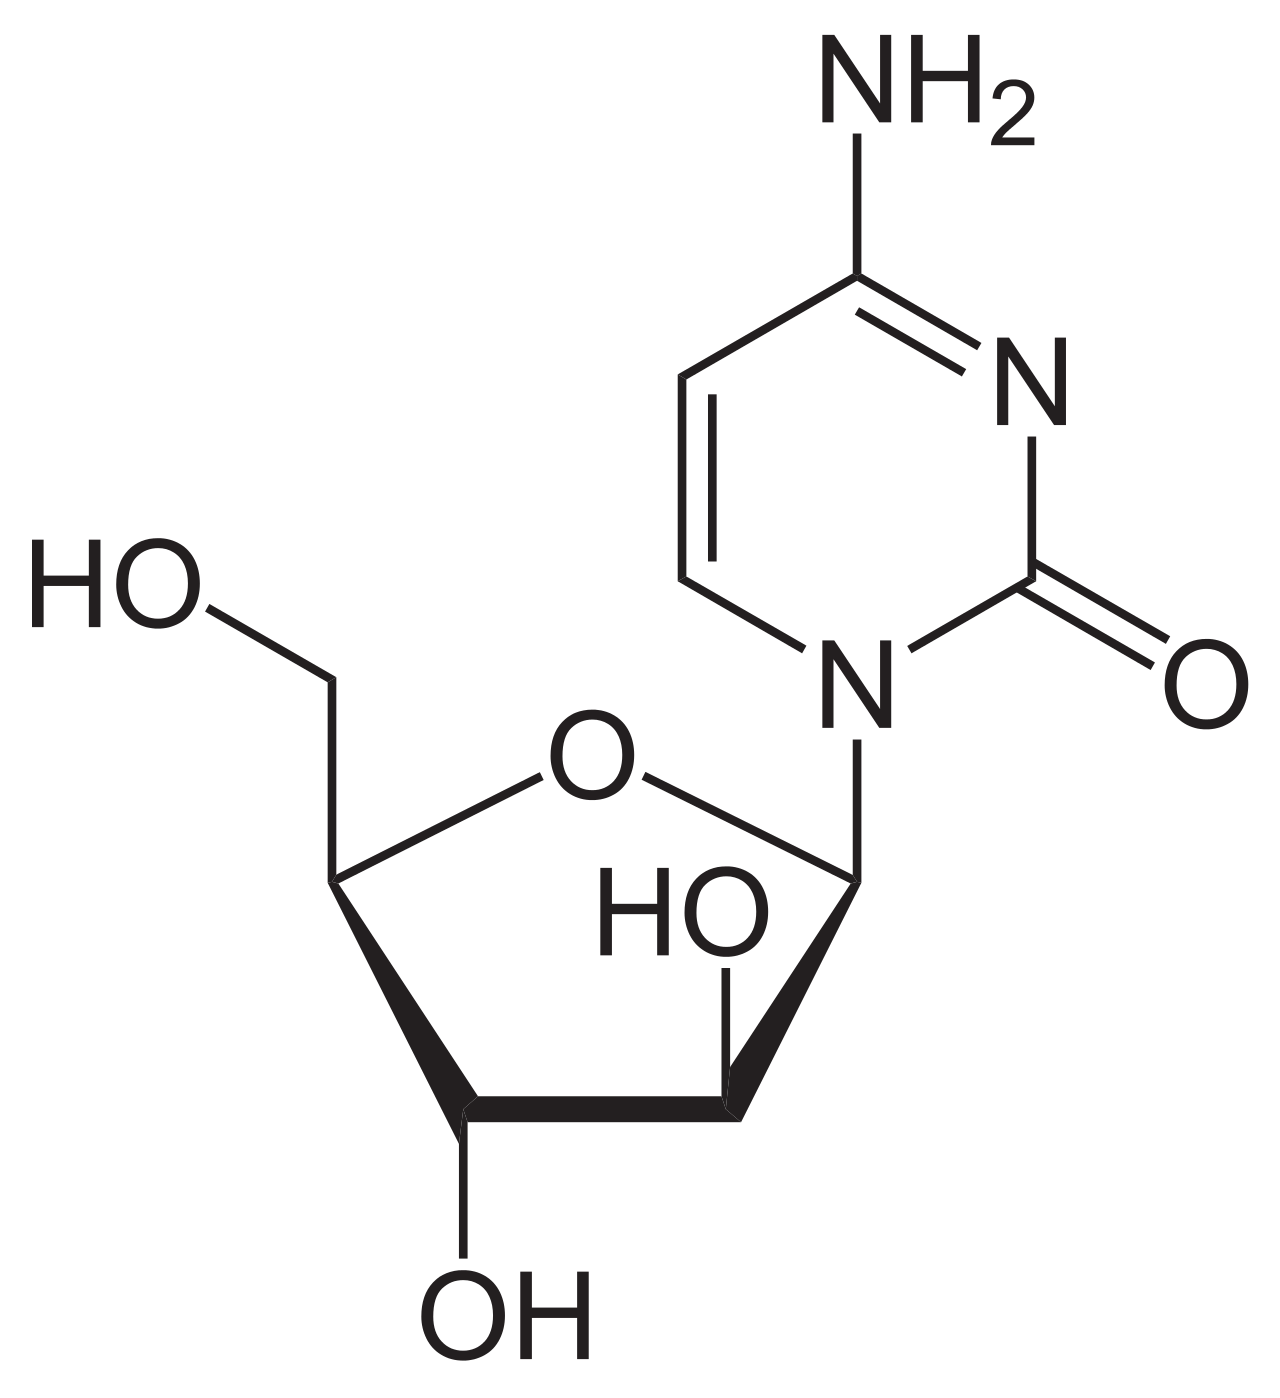
\includegraphics[scale=0.1]{Cytarabin.png}
	\caption{Molecular structure of chemotherapeutic drug Cytarabine}
	\label{fig:Cyt}
\end{figure}

